\subsection{ Fourier transform of a recorded signal }
For this task we are interested in analyzing a sample of a piano note in the
frequency domain, so that we may resynthesize it.

We load in the piano wave file by \emph{Matlab} code:
\begin{lstlisting}[
style=Matlab-editor,
basicstyle=\ttfamily,
numbers=none]
[piano, pianoFs, pianoNbits] = wavread( 'piano.wav' );
\end{lstlisting}


\subsubsection{ Original signal, time domain }
First we plot one second (from 0s-1s) of the original signal in the time domain
(\ref{fig:1-3-1s}).
A plot of the signal zoopmed in on a few periods is also provided in
(\ref{fig:1-3-period})

\begin{figure}
	\center
	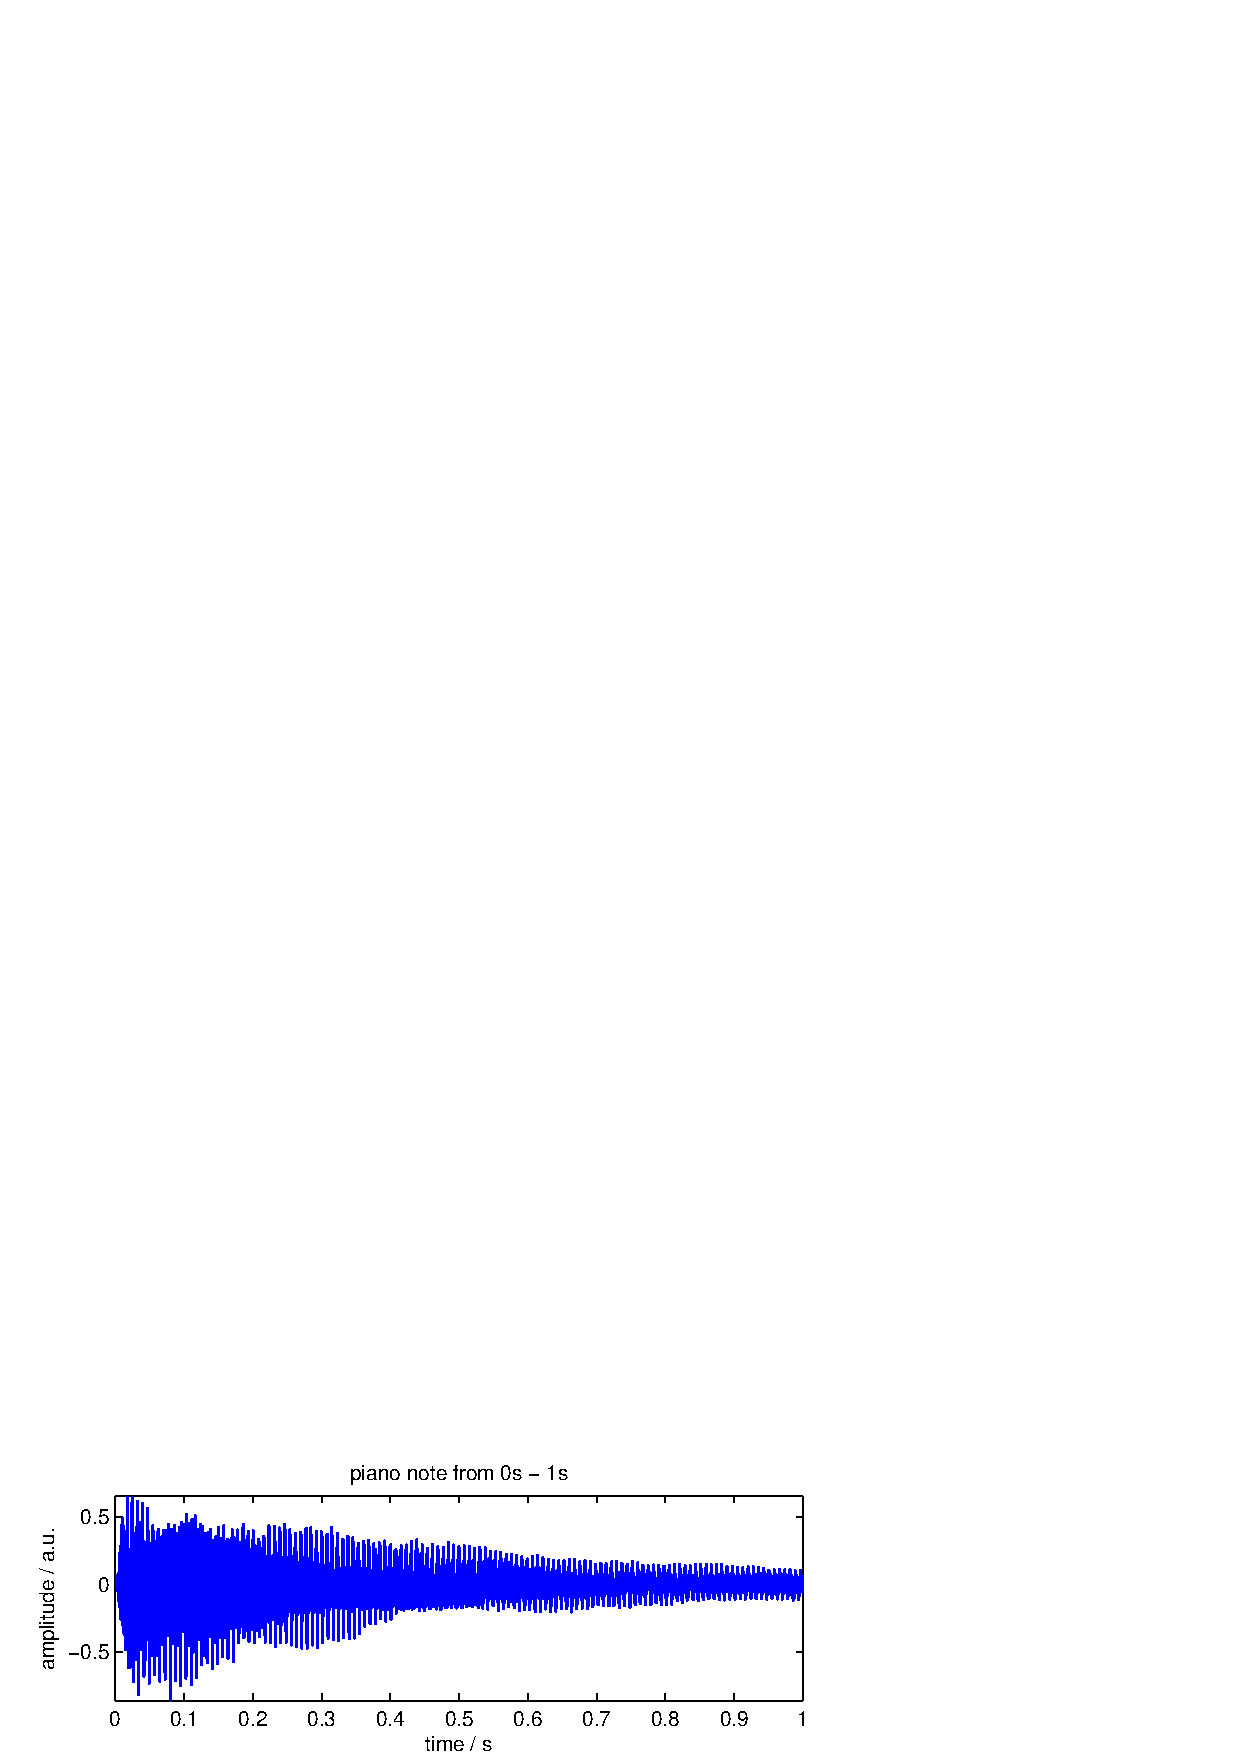
\includegraphics{1-3-1s}
	\caption{ Waveform of a piano note }
	\label{fig:1-3-1s}
\end{figure}

\begin{figure}
	\center
	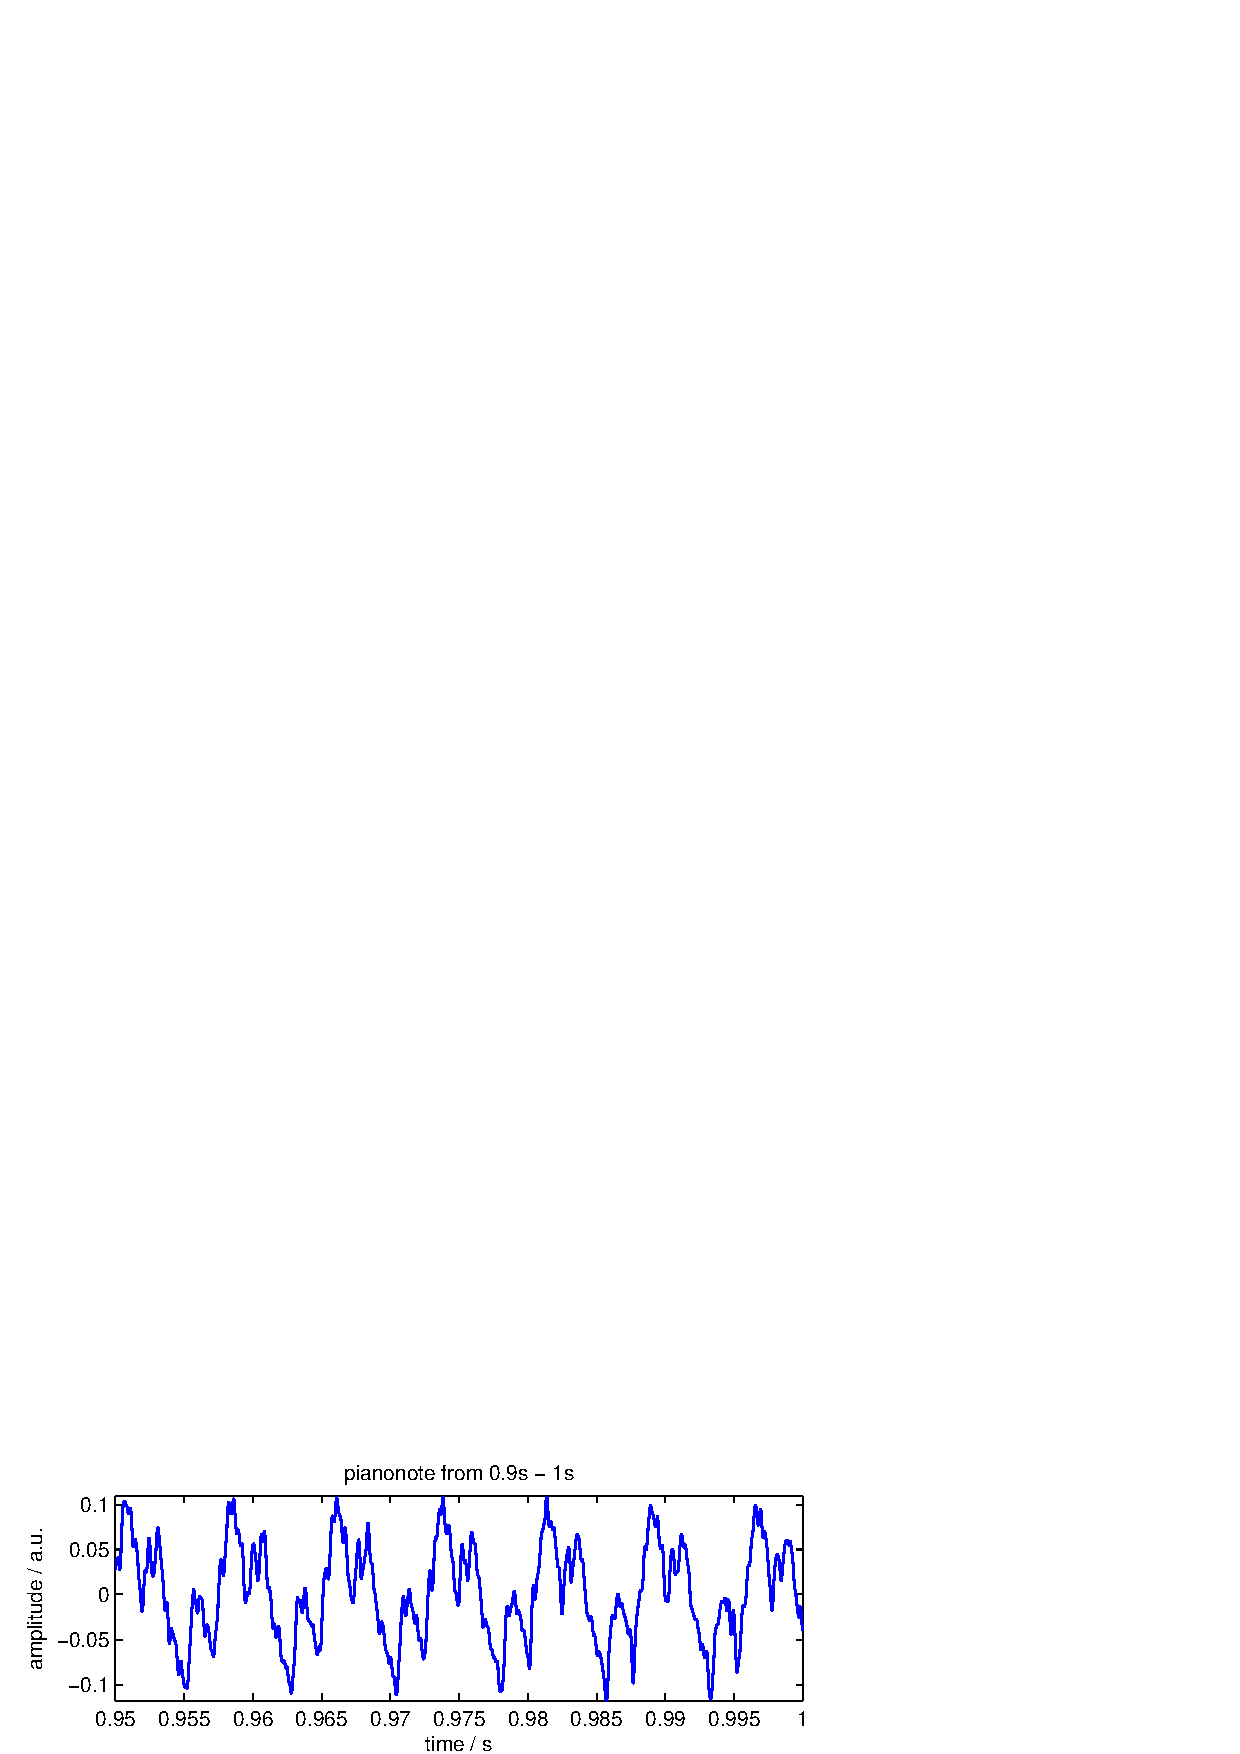
\includegraphics{1-3-period}
	\caption{ Zoom of piano note waveform }
	\label{fig:1-3-period}
\end{figure}

\subsubsection{ Original signal, frequency domain }
Using the previously described function \emph{make\_spectrum} we calculate the
spectrum of the piano signal.
\begin{lstlisting}[
style=Matlab-editor,
basicstyle=\ttfamily\footnotesize,
numbers=none]
% * Plot spectrum of whole signal on double log axis
[ Y, F ] = make_spectrum( piano, pianoFs );
% normalize fft
Y = Y / length(Y) * 2;
\end{lstlisting}

We then plot the spectrum of the positive
frequencies with magnitude in dB on the y axis and frequency in Hz on the x axis. Two plots are provided, one with
logarithmic x axis (\ref{fig:1-3-log}) and one with linear x axis
(\ref{fig:1-3-lin}). In (\ref{fig:1-3-lin}) we see how the overtones are almost
equally spaced.

\begin{figure}
	\center
	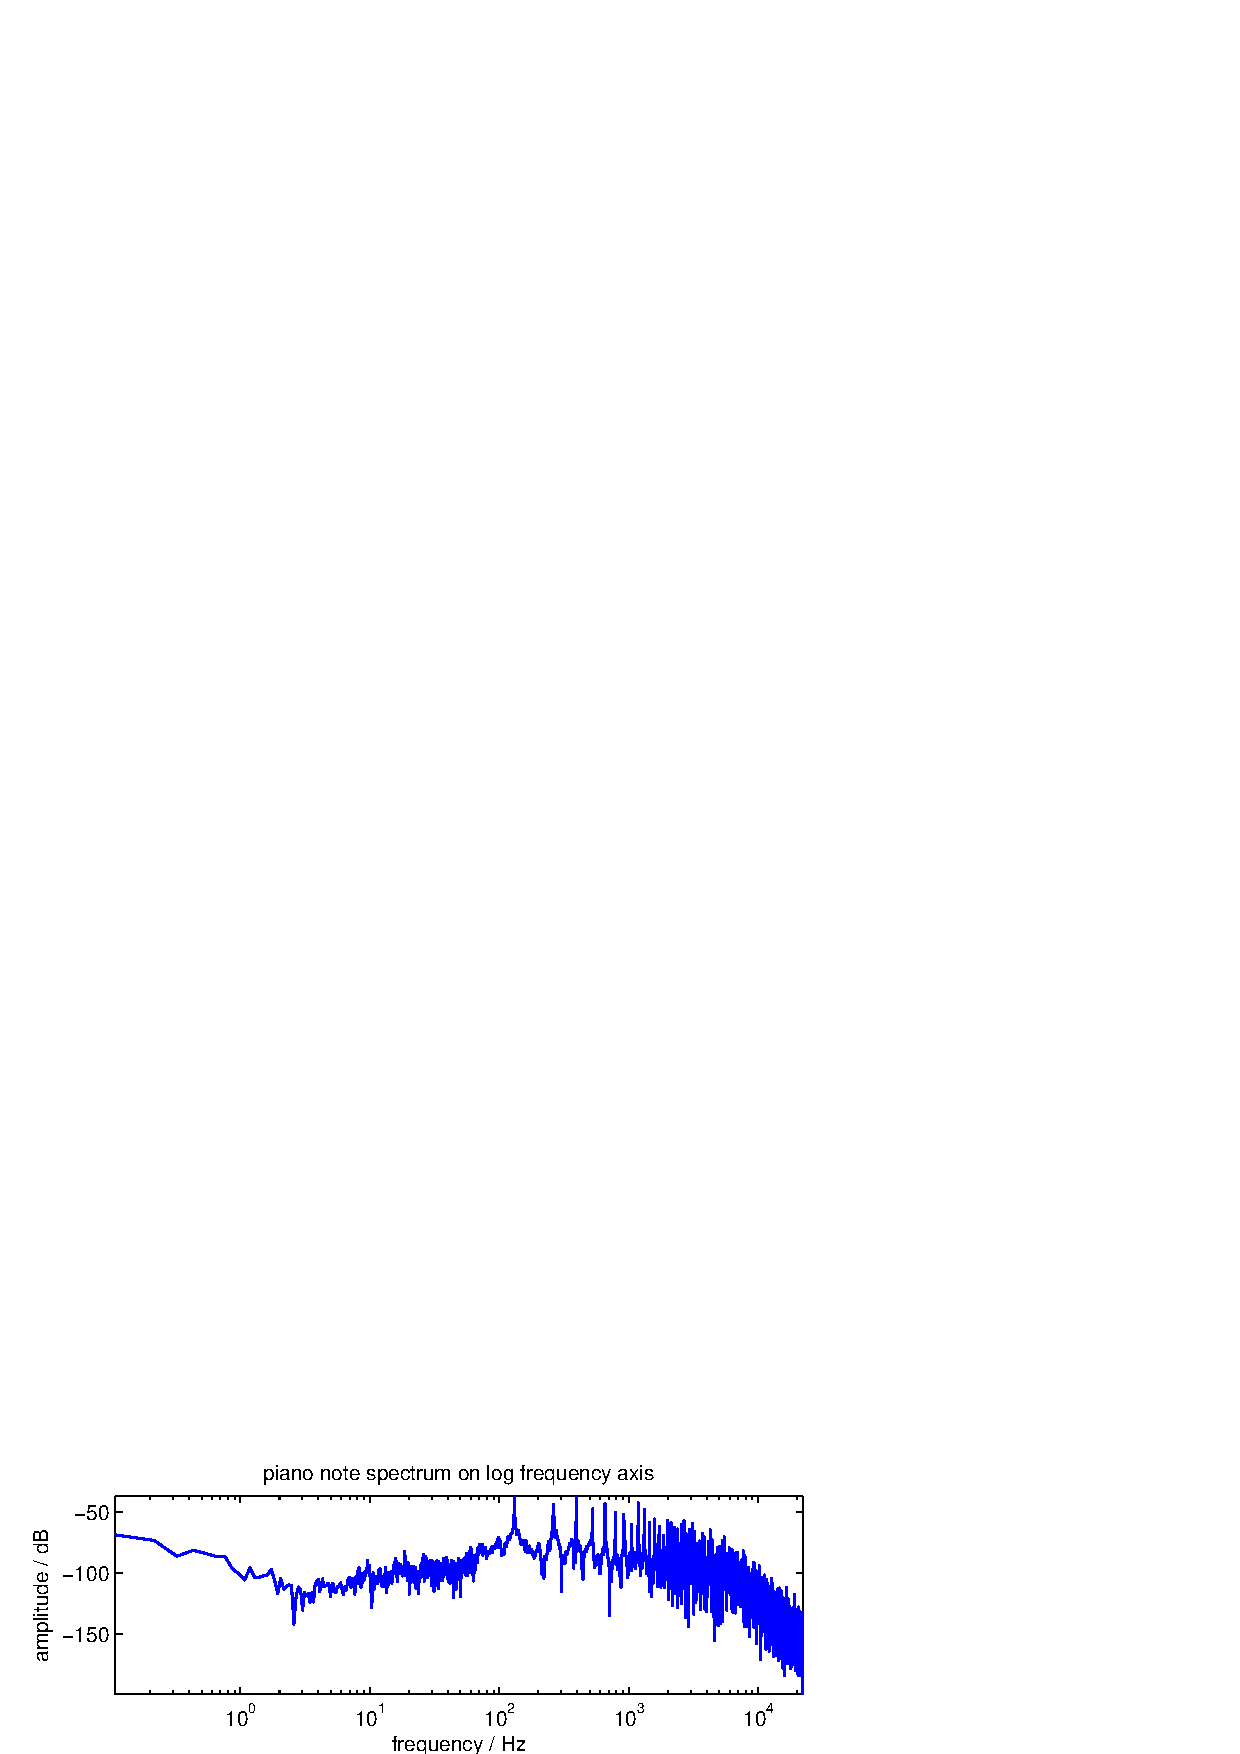
\includegraphics{1-3-log}
	\caption{ Spectrum of a piano note with a logarithmic frequency
axis }
	\label{fig:1-3-log}
\end{figure}	

\begin{figure}
	\center
	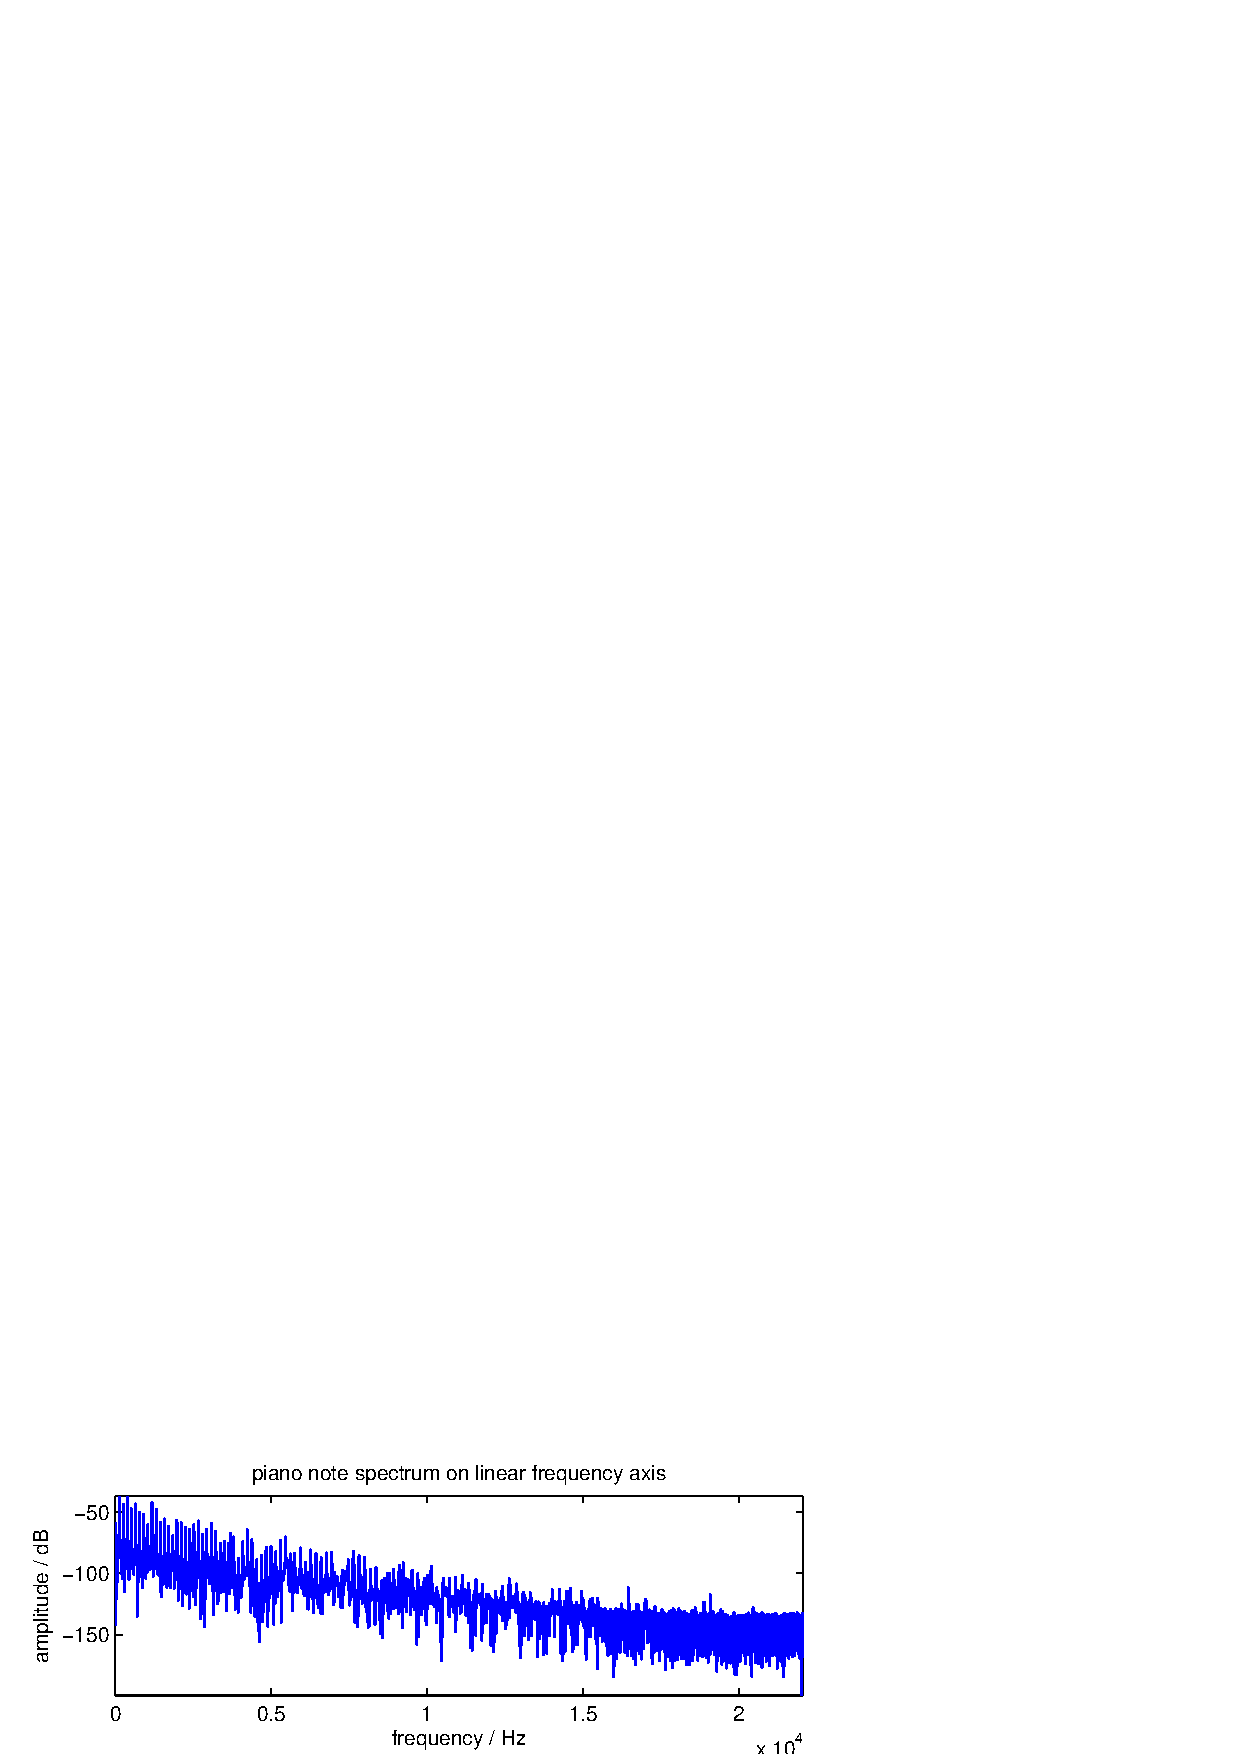
\includegraphics{1-3-lin}
	\caption{ Spectrum of a piano note with a linear frequency
axis. Notice how the harmonics are almost equally spaced }
	\label{fig:1-3-lin}
\end{figure}

\subsubsection{ Extracting frequency at peak magnitudes }
By plotting the spectrum with magnitude along y axis and inde along x axis, one
can use the \emph{Matlab data curser} in the figure window to get the exact
index of peak magnitudes.
\begin{lstlisting}[
style=Matlab-editor,
basicstyle=\ttfamily\footnotesize,
numbers=none]
% * plot with index along x to extract index of peak freq.
plot( mag2db(abs(Y(1:end/2))) )
% Set custom data curser callback. New callback increases resolution on
% readout to 10 decimals (instead of 4)
set(datacursormode,'UpdateFcn',@curserUpdate10);
\end{lstlisting}

This can be used to generate a vector of frequencies and magnitudes for re
synthesis.

\begin{lstlisting}[
style=Matlab-editor,
basicstyle=\ttfamily\footnotesize,
numbers=none]
peakIndex = [ 1211, 2424, 3639, 4853, 6064, 7284, 8503, 9725, 10950, 12178, ...
   13409, 14637, 15883, 17130, 18382, 19629, 20893, 22155, 23434, 24707, ...
   25997, 27285, 28592, 29898, 31216, 32538, 34264, 35219, 36579, 37963, ...
   39310, 40685 ]; 
freqVect = F( peakIndex );
amplVect = abs( Y( peakIndex ) );
% get base freq
f_0 = freqVect(1)
\end{lstlisting}
(Note the choise of 32 readings was semi random, but too few and the
resynthesized signal sounds like an oboe or clarinet. Since $32\cdot f_0
\approx 4000\mbox{Hz}$ and the amplitude of the $31^{st}$ overtone is roughly
$30\mbox{dB}$ under that of $f_0$ this seemed reasonably. )

This gives us a fundamental frequency of $130.43\mbox{Hz}$, very close to a
$C3$.

\subsubsection{ Resynthesis }
A function is made to generate a discrete fourier series from a vector of
frequencies and complex magnitudes. Given a desired frequency resolution and
sample rate, the closest frequency resolution resulting in an integer number of
samples in the fourier domain is chosen. Each magnitude is then put into the bin
closest to the coressponding frequency:
\begin{lstlisting}[
style=Matlab-editor,
basicstyle=\ttfamily\footnotesize,
numbers=left]
function [ synFreq, F ] = generateSpectrum( freqVect, amplVect, dF, fs )
%GENERATE_SPECTRUM genereates the spectrum from a list of frequencies and
%amplitudes that fits the best into the spectrum of resolution dF
%   freqVect and amplVect is the frequency and amplitude vectors
%   dF is the desired spectrum resolution
%   fs is the sample frequency

% choose nearest dF, that gives an integer number of samples:
dF =  fs / round(fs/dF);

% generate a vector of zeros for us to set the magnitudes in:
synFreq = zeros( round(fs/dF), 1 );

% set bin value for the bin closest to each specified frequency:
for i = 1:length(freqVect)
    % positive frequency
    synFreq( 1 + round((freqVect(i))/dF) ) = amplVect( i )/2;
    % negative frequency
    synFreq( end + 1 - round((freqVect(i))/dF) ) = conj(amplVect( i )/2);
end

% genreate frequeny vector
F = ( 0 : dF : fs - dF )';
F(ceil(end/2)+1:end) = F(ceil(end/2)+1:end) - fs;

end
\end{lstlisting}

We also costruct a wrapper function for generating the time signal from a
fourier series and extend/truncate it to a desired length:
function [ synTime, T ] = spect2time( synFreq, fs, len )
\begin{lstlisting}[
style=Matlab-editor,
basicstyle=\ttfamily\footnotesize,
numbers=left]
%SPECT2TIME Genreates a timeseries signal from spectrum synFreq and
%   extends/truncates to length

synFreq = synFreq*length(synFreq);

% generate time signal
synTime = ifft( synFreq );

% resize signal
synTime = repmat( synTime, ceil( fs*len/length(synTime) ), 1 );
synTime = synTime(1:fs*len);

%genreate time vector
T = 0:1/fs:length(synTime)/fs-1/fs;

end
\end{lstlisting}

We are now ready to resynthesize the signal in the time domain.
\paragraph{ Resynthesis assuming zero-phase and perfect harmony }
First we try to resynthesize the piano note assuming that all overtones are
perfect harmonics (multiples) of the fundamental frequency, that is the
frequency vector is given by:
\begin{equation*}
 f_0, 2 f_0, 3 f_0, \ldots , 31 f_0
\end{equation*}
and all frequencies are in phase.
We choose a frequency resolution of $0.01\mbox{Hz}$ since this results in an
integer number of frequency bins and also enables us to place the harmonics
without rounding off their position.

The magnitude vector is given by the absolute of each of the original
magnitudes.

Again we plot a couple of periods of the signal. This is done in
(\ref{fig:1-3-zpph_time}). We also plot the spectrum of both the synthesized
signal an the original signal from 0 to 4500Hz to compare them in
(\ref{fig:1-3-zpph_fft}). You can see that after the first ~10 harmonics, the
frequency of the synthesized harmonics and the original starts to deviate. This
is note simply a result of choosing $f_0$ with too low resolution, but the
harmonics actually aren't perfect.

\begin{figure}
	\center
	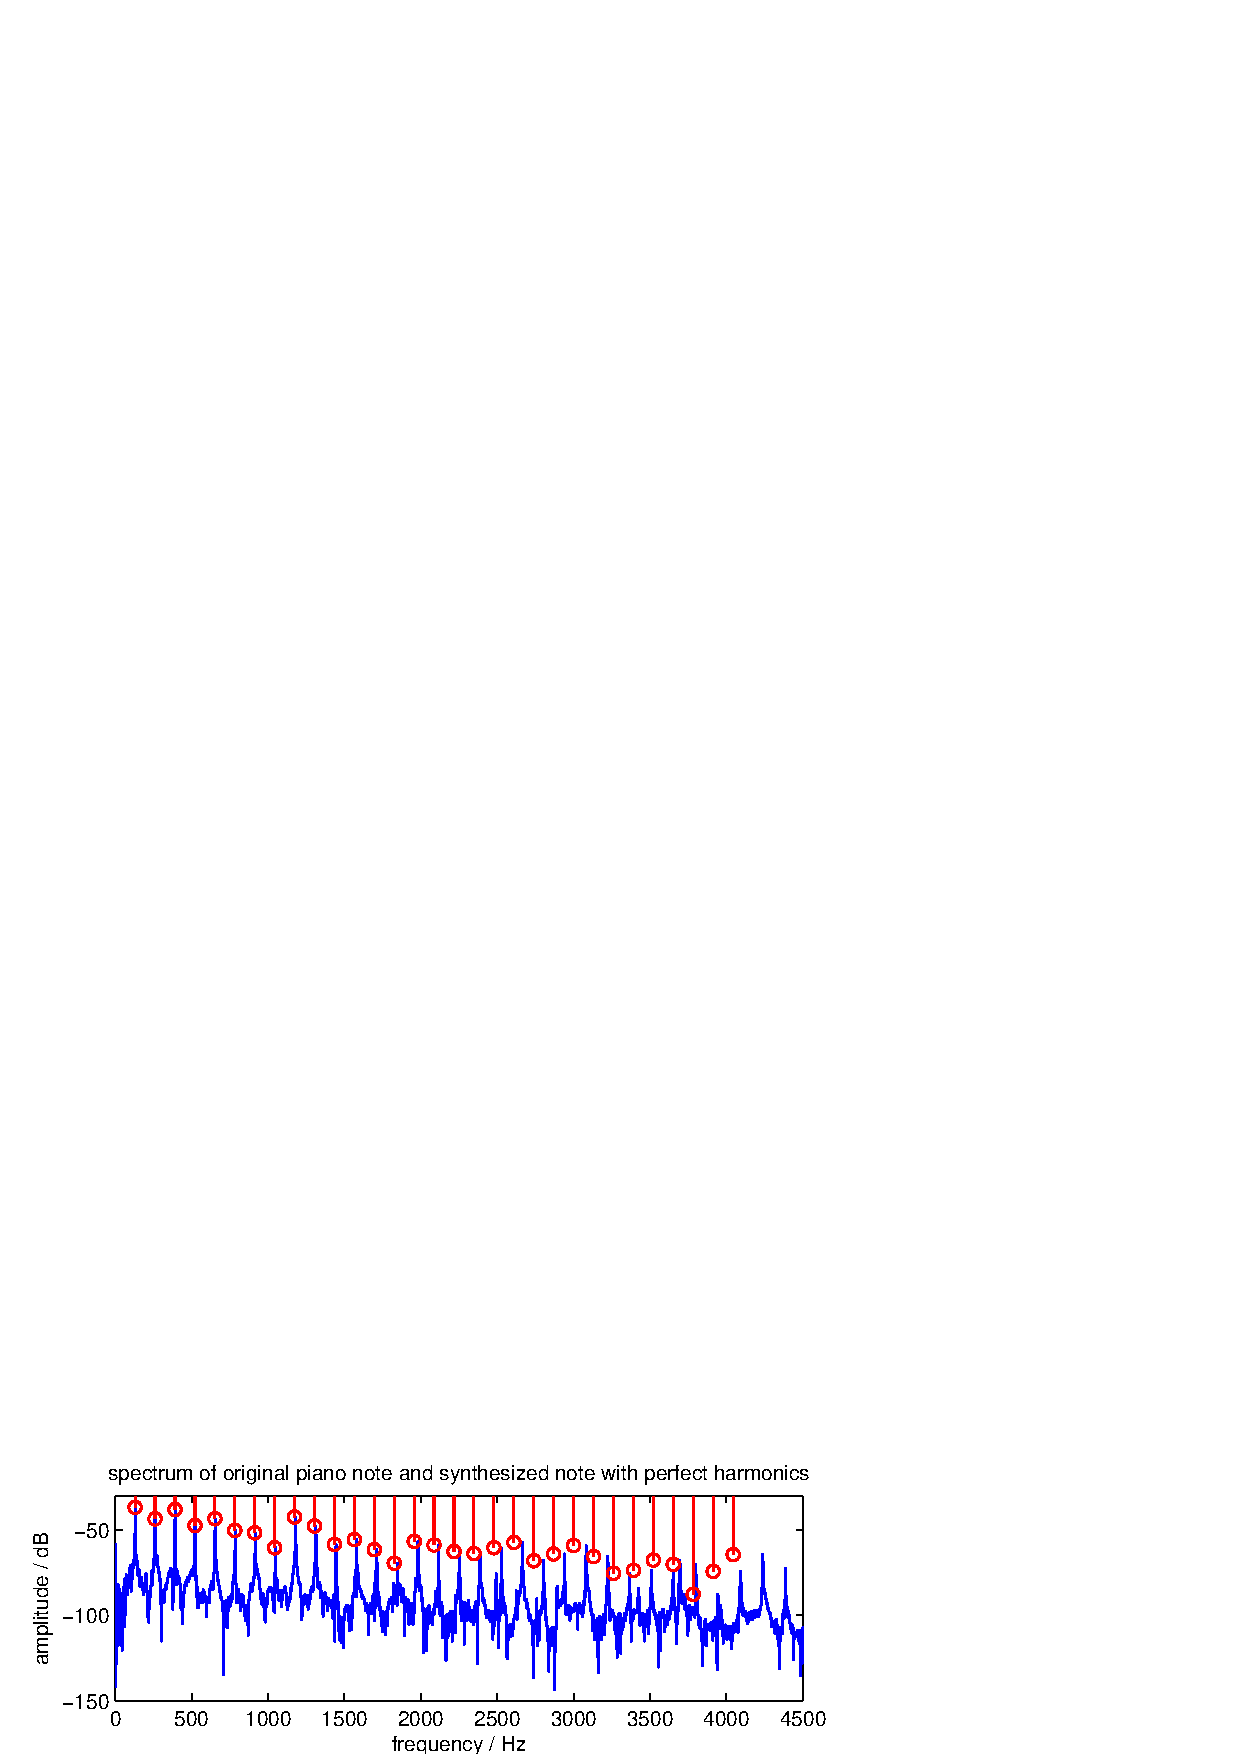
\includegraphics{1-3-zpph_fft}
	\caption{ Original spectrum overlayed i with synthesized
spectrum for perfect harmonics. Notice how the overtones aren't perfect
harmonics }
	\label{fig:1-3-zpph_fft}
\end{figure}

\begin{figure}
	\center
	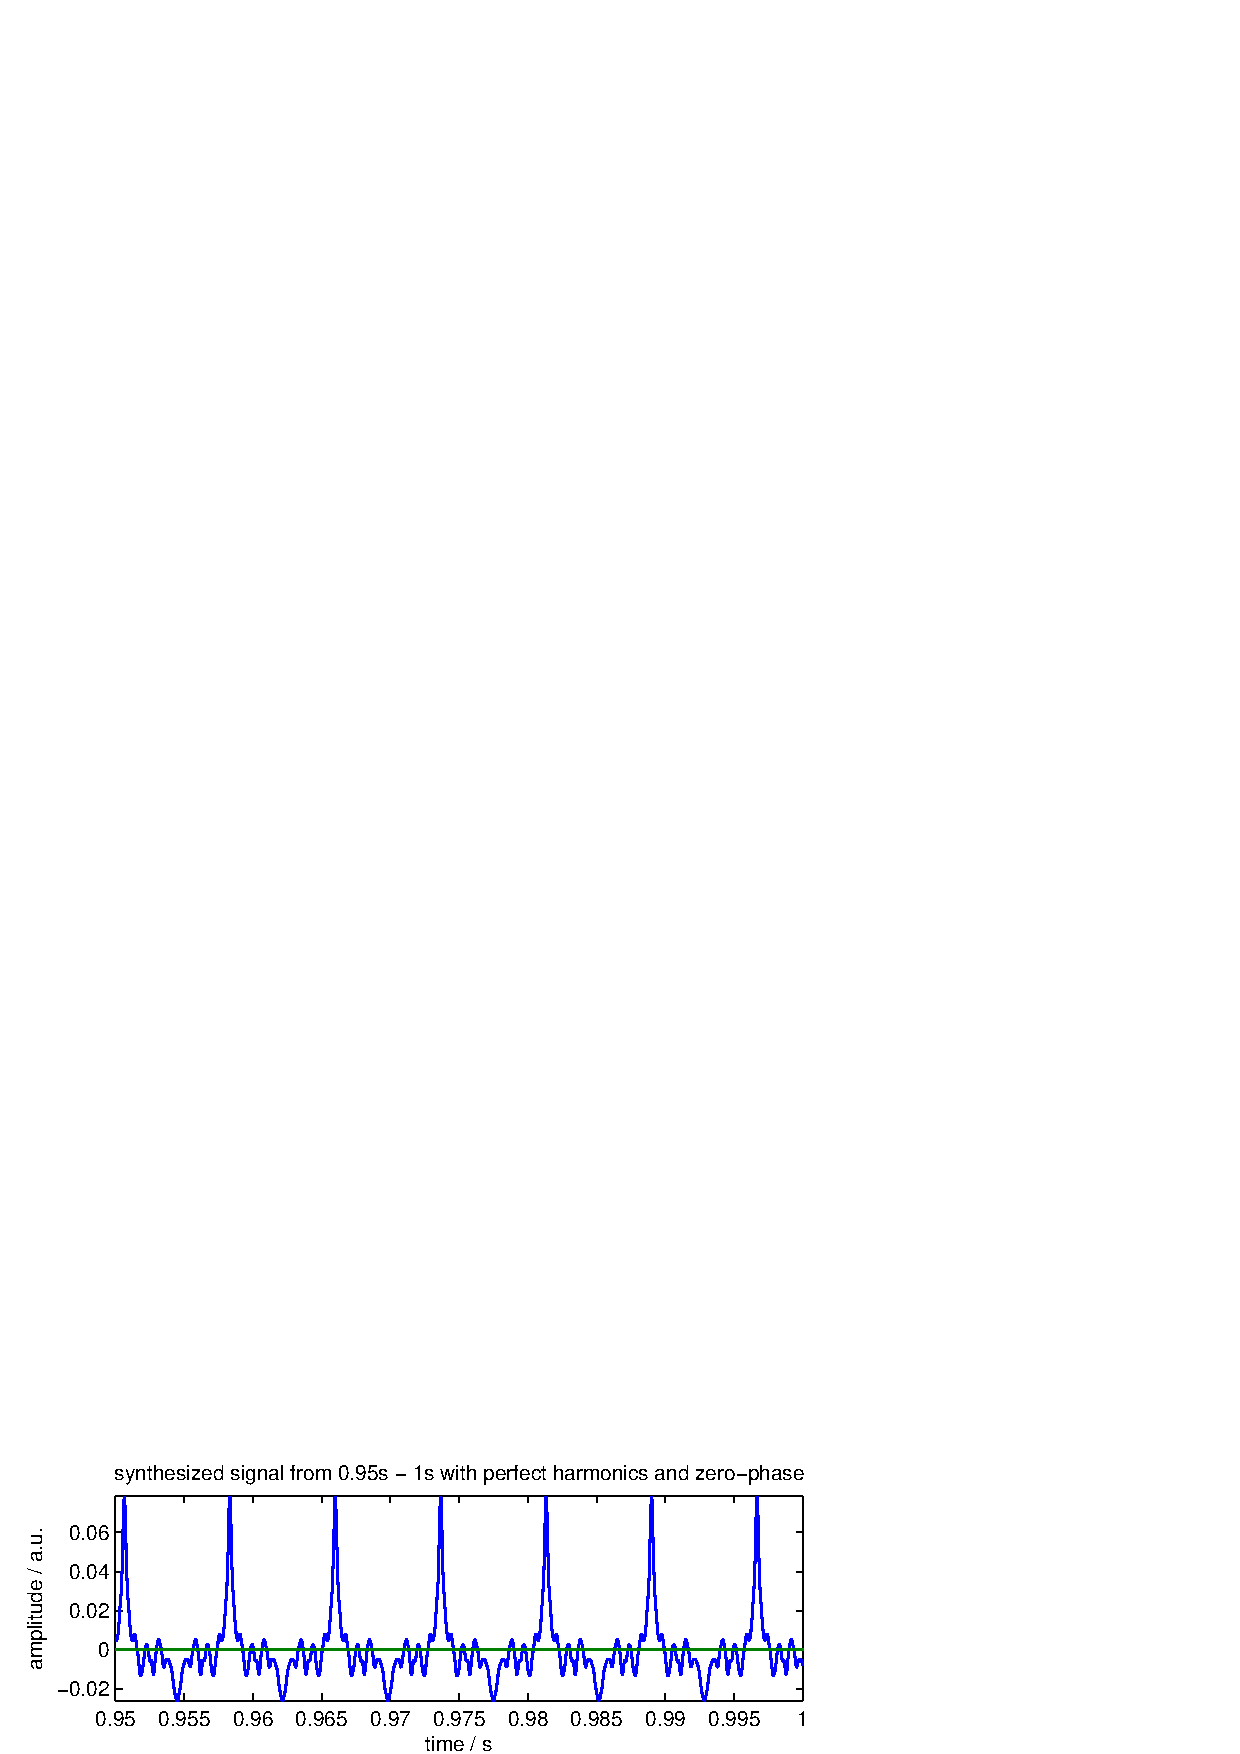
\includegraphics{1-3-zpph_time}
	\caption{ Zoom on the synthesized signal, assuming perfect
harmonics and same phase for all overtones }
	\label{fig:1-3-zpph_time}
\end{figure}


\paragraph{ Resynthesis with correct phase and perfect harmony }
We then resynthezise in the same manner, but using the complex magnitude.
A couple of periods of the signal can be seen in
(\ref{fig:1-3-nzpph_time})

Listening to the two signals, there is a sligt difference.
The signal with complex magnitude sounds slightly more nasal and perhaps a bit
closer to the original.

\begin{figure}
	\center
	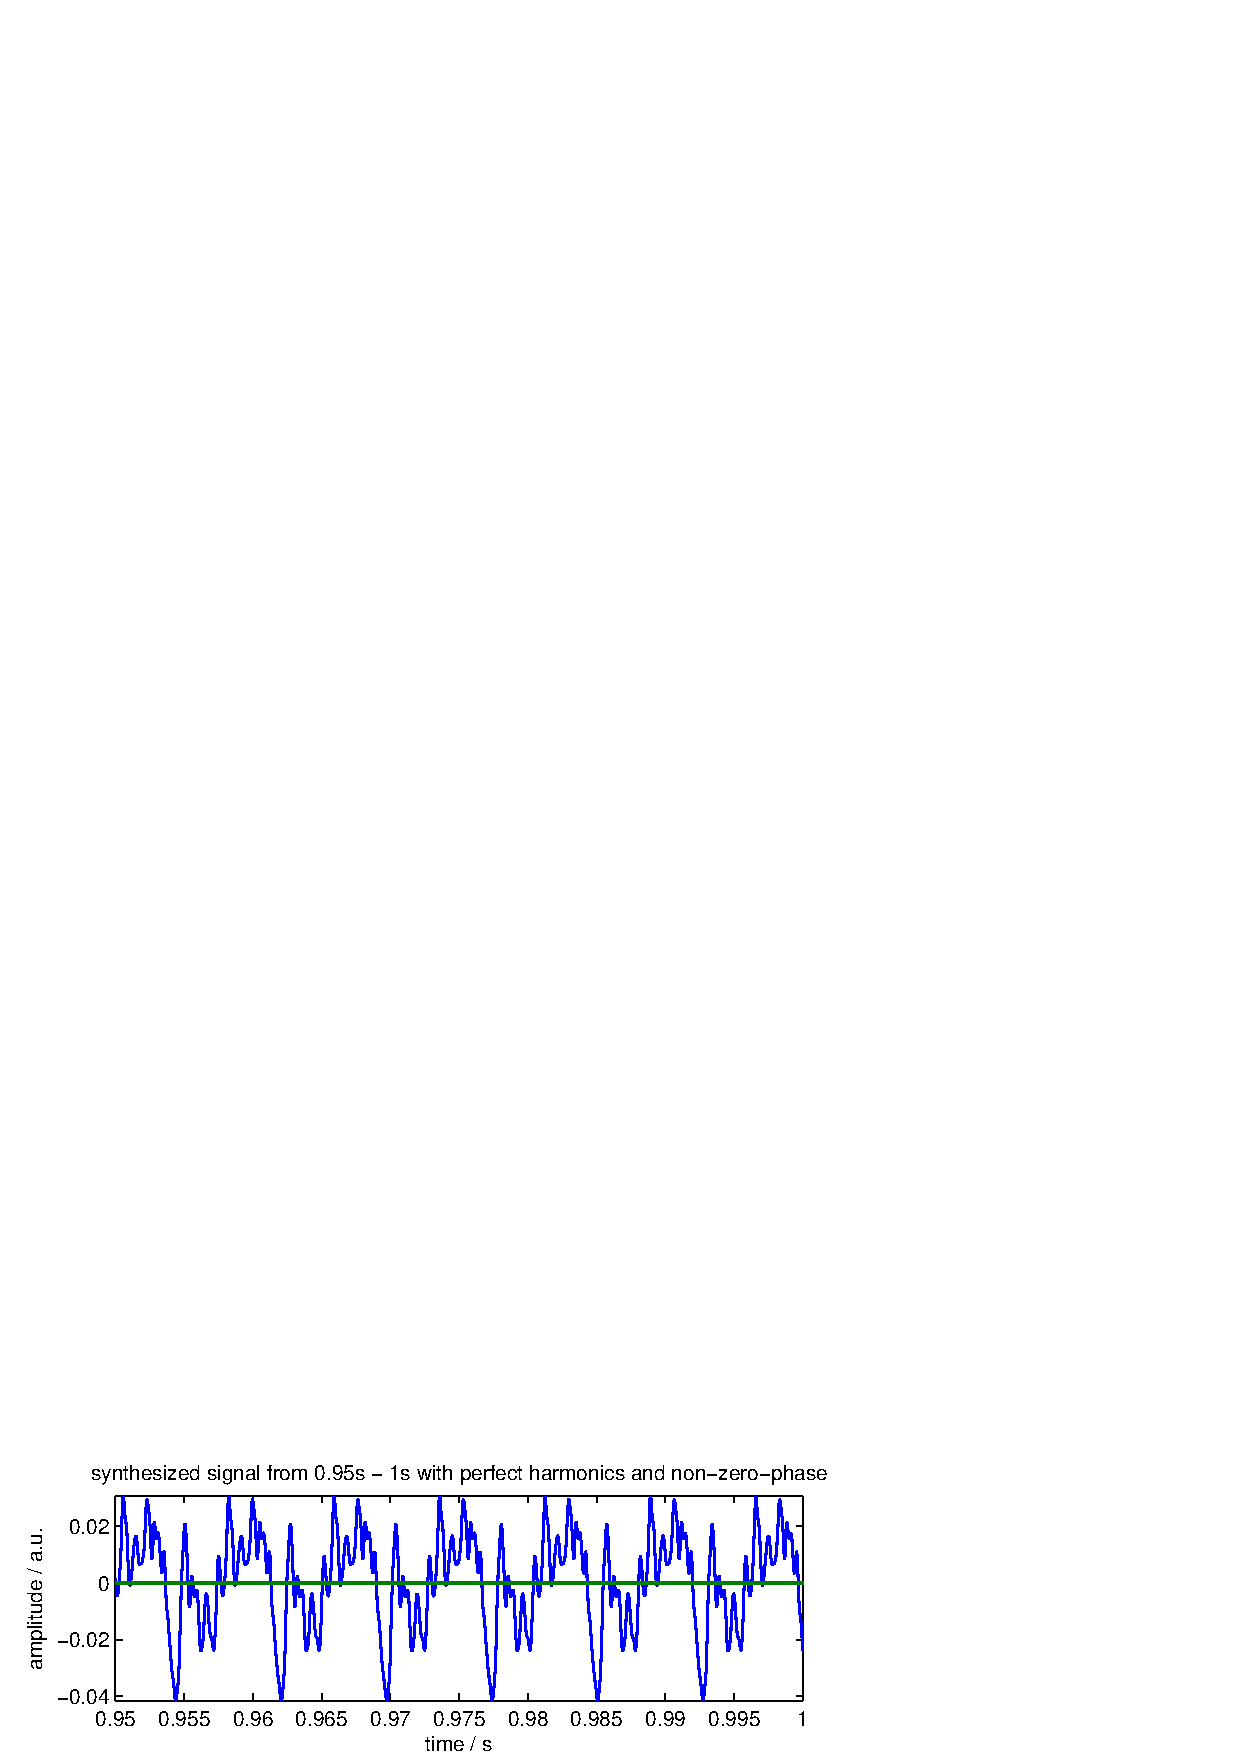
\includegraphics{1-3-nzpph_time}
	\caption{ Zoom on the synthesized signal, assuming
 perfect harmonics and correct phase for the overtones. }
	\label{fig:1-3-nzpph_time}
\end{figure}

\paragraph{ Resynthesis with correct phase and imperfect harmony }
To get even closer to the real piano we also have to recreate the slight beating
produced by the harmonics not being perfectly multiples of $f_0$,
this is done using the original frequency vector (\emph{freqVect}) and complex
phase vector. In (\ref{fig:1-3-nzpih_fft}) we see how the spectrum of the
synthesized signal now matches the original.

In (\ref{fig:1-3-nzpih_time}) we see how the waveform changes slightly over
time.
Playing this file, we can hear that it is even closer, as it has got some of the
``life'' back, pulsing slightly. Now all we need is an envelope generator to
recreate the onset of the note.

\begin{figure}
	\center
	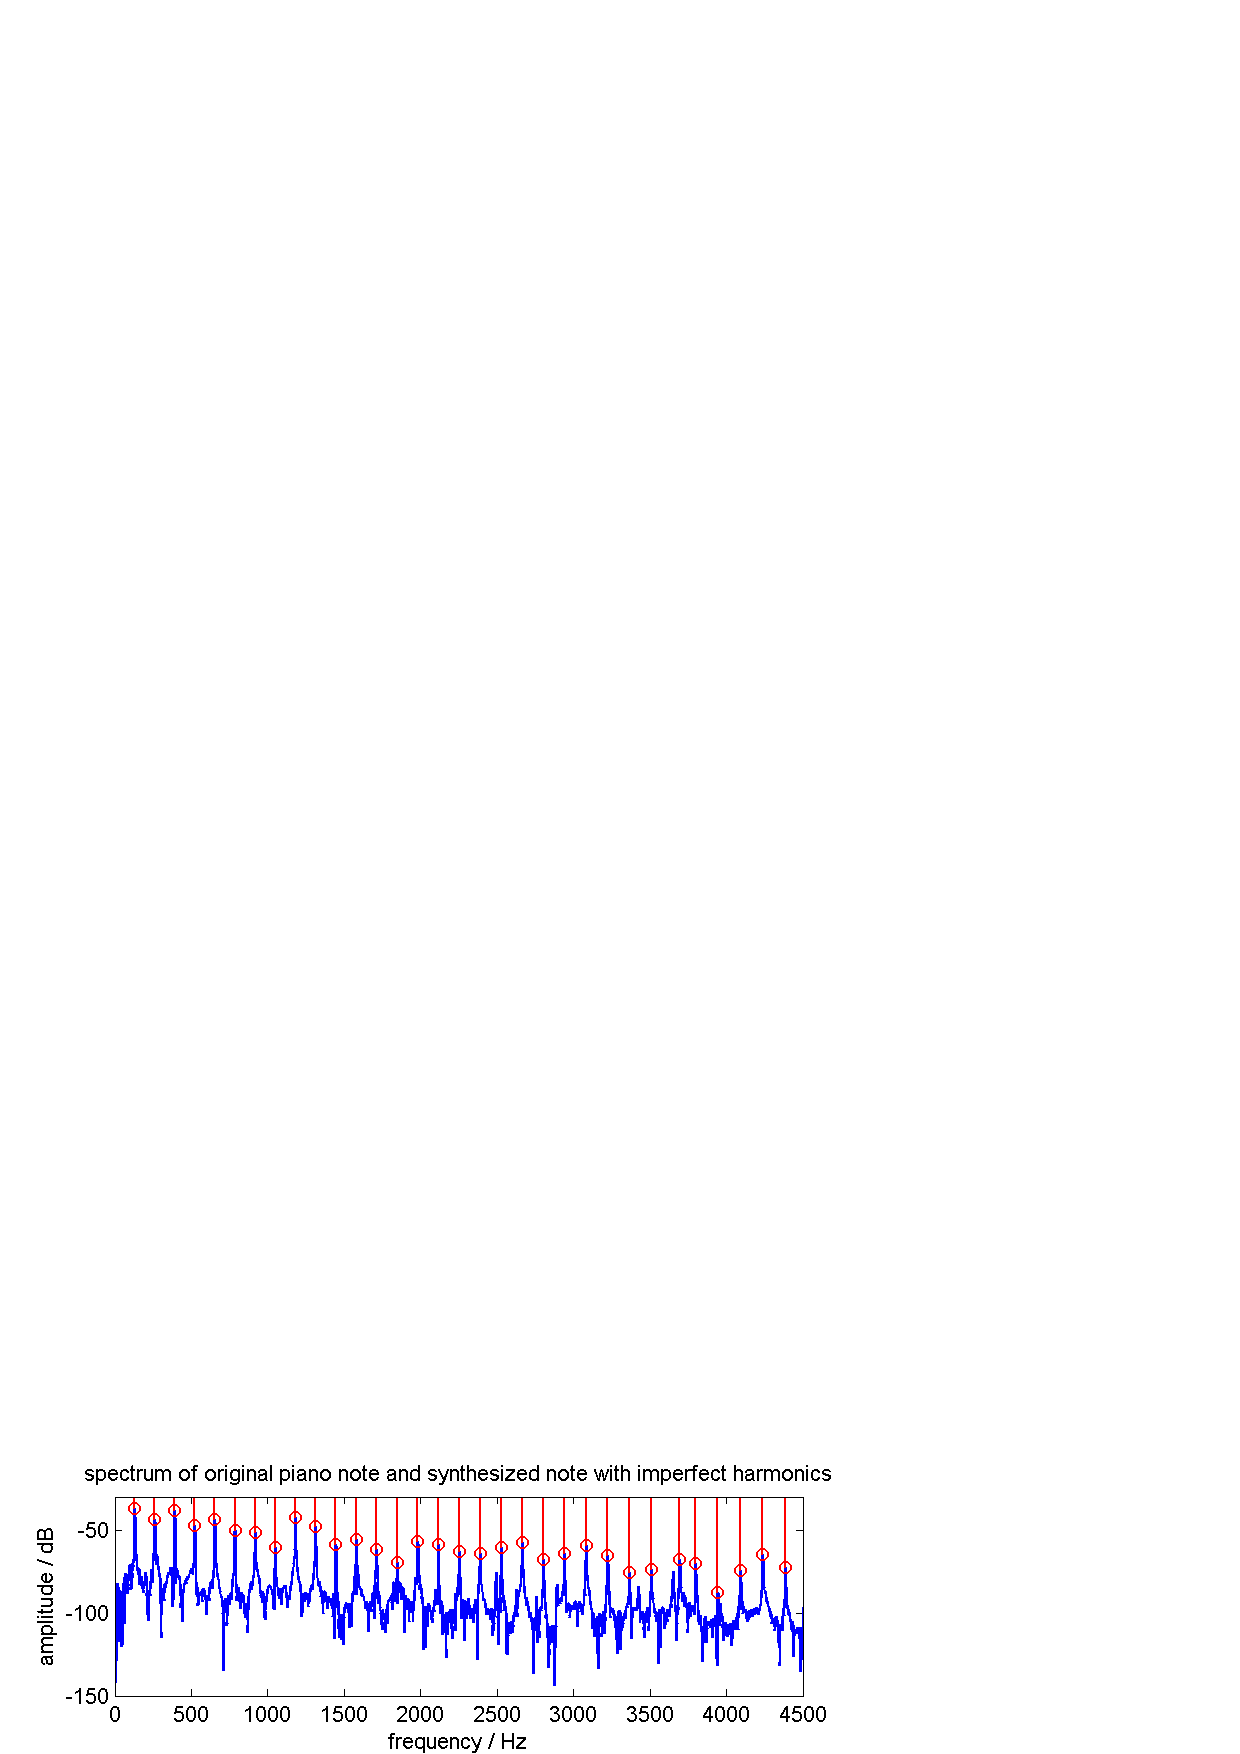
\includegraphics{1-3-nzpih_fft}
	\caption{ Original spectrum overlayed i with synthesized
spectrum. Notice how the synthesized overtones now overlap with the original
overtones. }
	\label{fig:1-3-nzpih_fft}
\end{figure}

\begin{figure}
	\center
	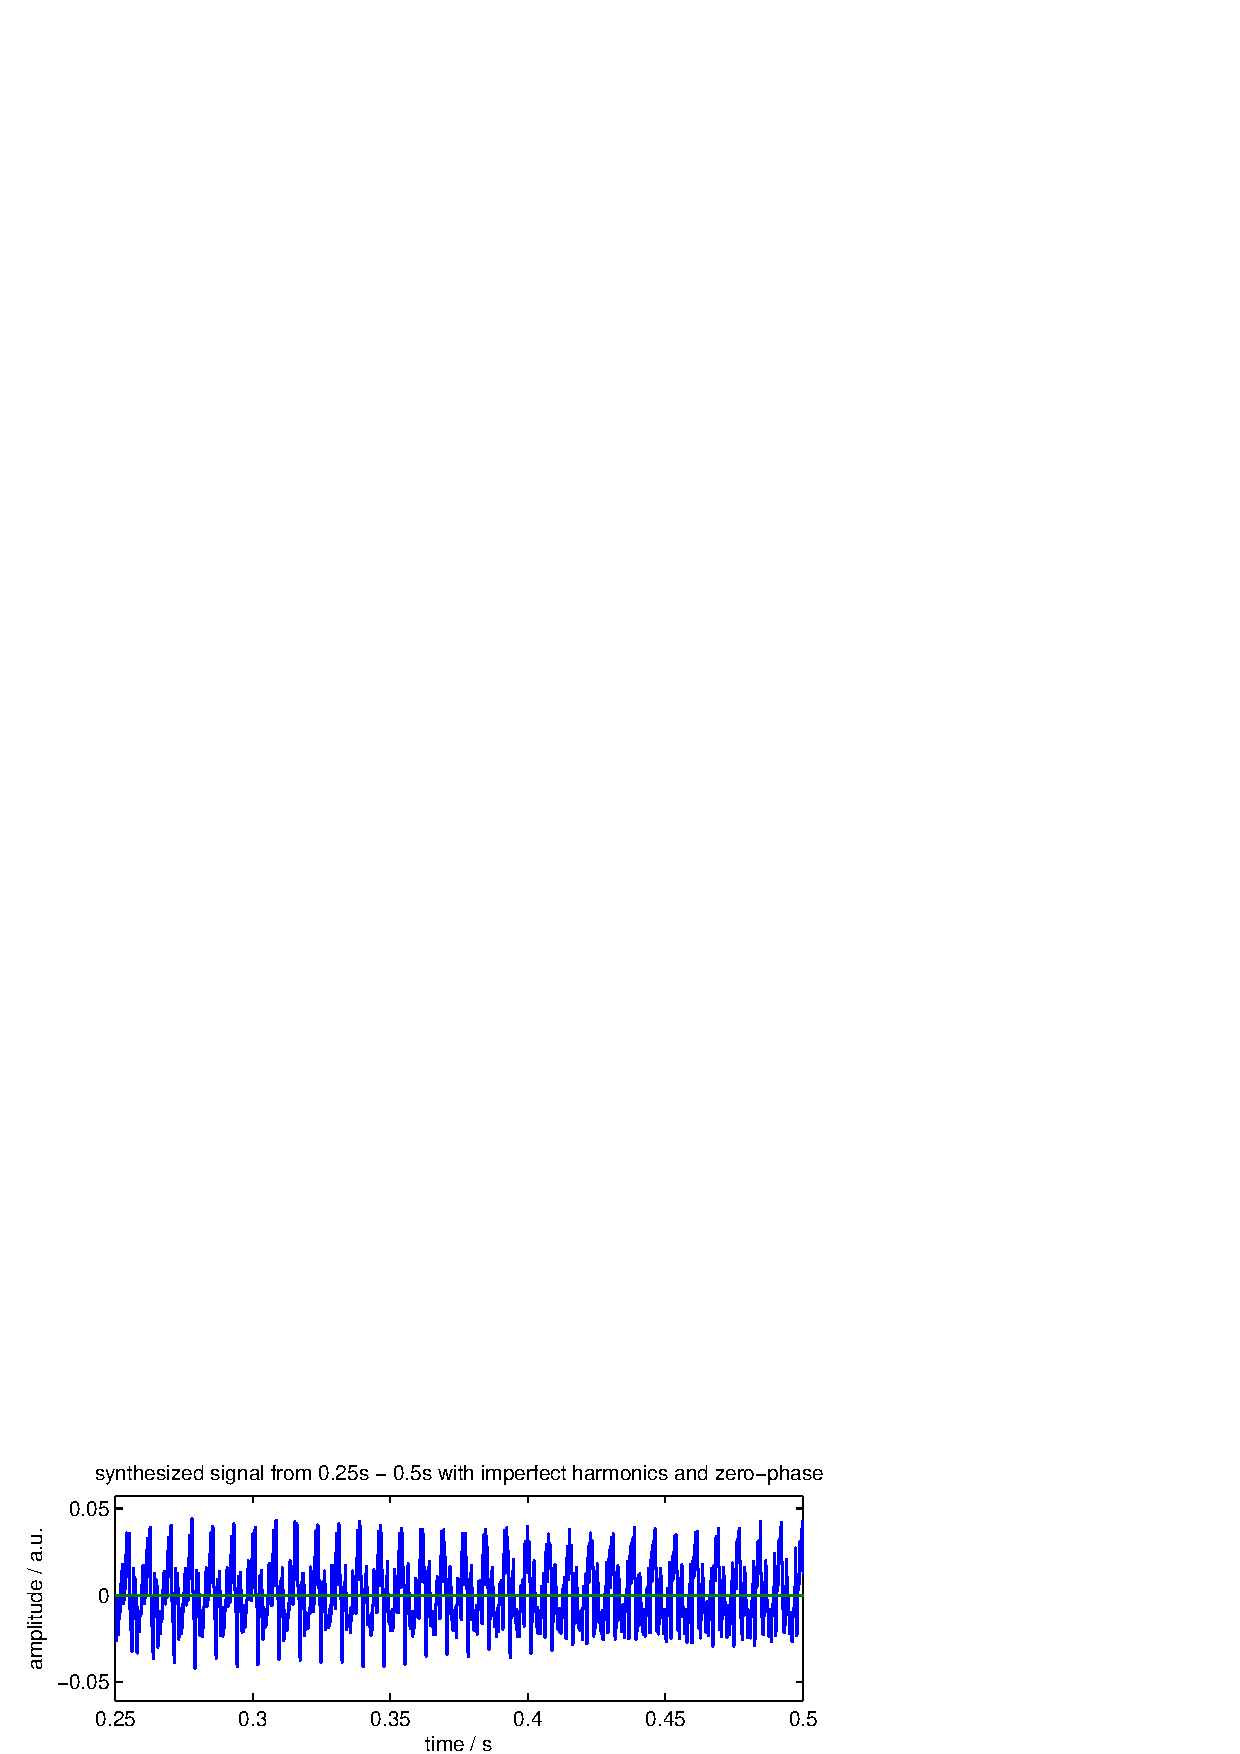
\includegraphics{1-3-nzpih_time}
	\caption{ Synthesized signal with
non-harmonic overtones. Notice how the shape of the
waveform changes over time }
	\label{fig:1-3-nzpih_time}
\end{figure}
